
%*******************************************************************************
%***********************************    Background   *****************************
%*******************************************************************************
%!TEX root = 0.main.tex

\setcounter{page}{1}



%********************************** %First Section  **************************************
\section {Introduction and general background} 

\subsection{Introduction}

[Intro to neural networks]\\
Neural Networks are popular algorithms for regression and classification tasks. In complex problems where we don't know the important features of the input data, neural networks can automatically "learn" these features through multiple combinations of linear and non-linear transformations of the input. Taking for example an image classification task, the first "layer" of a neural network transforms the input image in a vector that is given as input to the following layer, and so on, until the original image is mapped into a class by the last layer of the neural network. A neural network is capable of learning the optimal transformations that let it map the input image to the correct class. Since these transformations are parametrized by millions of parameters, a neural network is able to learn very complex transformations, characteristic that makes them the optimal tool for complex tasks such as image classification, image segmentation, speech recognition and natural language processing.\\

[Intro to CNN]\\
Convolutional Neural Networks (CNNs) are a specific class of neural networks whose layer structure has been specifically designed for image recognition and segmentation. For this purpose, they don't have all the degrees of freedom of a normal, "fully connected" neural network described above: each layer of a CNN has been constrained to only learn transformations of the input that are equivariant to translation of the input. This means that if used in an image classification task, a translation of the input image will not result in a change of class. To be specific, the transformation that each layer of a CNN performs is a \textit{convolution} of the input vector with a kernel. It is this kernel that is learned during the training phase. Thanks to their design, training of CNNs is faster - thanks to the smaller number of parameters to be learned compared to a fully connected neural network - easier -since there's no need of artificially augmenting the dataset with translated copies of the same image- and leads to very accurate results.\\

[Intro to Spherical CNN]\\
Spherical convolutional neural networks (SCNNs) are a variation of CNNs that have been designed to deal with spherical data, whose layer design make them equivariant to rotations of the input.  Examples of tasks where data is naturally represented on a sphere are (i) climate science, where data is sampled on the surface of the Earth, (ii) cosmology, where observations are naturally projected on a sphere centered around the observer (see Figure \ref{fig:cosmicradiation}), and (iii) virtual reality, where the images are represented on a sphere centered around the player. Being able to come up with designs that are equivariant to rotations brings to these tasks all the advantages that traditional CNNs have brought for traditional (euclidean) image classification tasks: training is faster, easier and results are very accurate. To be specific, the transformation that each layer of a SCNN performs is a \textit{spherical convolution} of the input vector with a kernel. It is this kernel that is learned during the training phase. 

\begin{figure}

	\centering
	\caption{\label{fig:cosmicradiation} Cosmic microwave background map, the oldest electromagnetic radiation in the universe. Source: Wikipedia}
	\includegraphics[width=0.4\textwidth]{figs/literaturereview/WMAP.png}
\end{figure}

[Intro to Graph CNN and DeepSphere]\\
One of the main issues with Spherical Neural Networks is the computational complexity of computing at each layer the spherical convolutions to learn the best kernel. Deferrard et al \cite{DeepSphere} proposed an architecture that is almost equivariant to rotations, but limit the computational complexity of the algorithm to be linear with the dimension of the input data. The idea is to construct a suitable graph connecting the pixels of the image, represent the image as a signal on this graph and then use at each layer \textit{graph convolutions} to approximate spherical convolutions.
\subsection{Fourier Transforms and Convolutions on the 2-Sphere}
[Review of \textit{Computing Fourier Transforms and Convolutions on the 2-Sphere}]
If we find a basis of minimal subspaces invariant (a vector space of functions on the sphere is invariant if all of the operators $\Lambda(g), g\in SO(3)$ take each function in the space back into the space) under all the rotations of $SO(3)$, then we simplify a lot the analysis of rotation-invariant operators.
\paragraph{Things to keep in mind from section 2, "Preliminaries"}
\begin{enumerate}
	\item any rotation $g\in SO(3)$ can be written in the well-known Euler angle decomposition: $g = u(\phi)a(\theta)u(\psi)$ determined uniquely for almost all $g$. Remember that any point on the sphere
	\item $\omega(\theta, \phi) = \left(\cos\phi\sin\theta, \sin\phi\sin\theta, \cos\theta\right)$. In fact, the 2-sphere is a quotient of the rotation group $SO(3)$ and inherits its natural coordinate system from that of the group.
	\item $\Lambda(g)f(\omega) = f(g^{-1}\omega)$
	\item invariant volume measure on $SO(3)$ is $dg=\sin\theta\ d\theta\ d\phi\ d\psi$, invariant volume measure on the sphere is $d\omega = \sin\theta\ d\theta\ d\phi$
	\item The invariant subspace of degree $l$ harmonic polynomials restricted to the sphere is called the space of \textit{spherical harmonics of degree l}. Spherical harmonics of different degree are orthogonal to one another
	\item In coordinates, 
	$$Y_l^m(\theta, \phi) =(-1)^m\sqrt{\frac{(2l+1)(l-m)!}{4\pi(l+m)!}}P_l^m(\cos\theta)e^{im\phi}$$
	where $P_l^m$ are Legendre functions.
	\begin{figure}
		\centering
		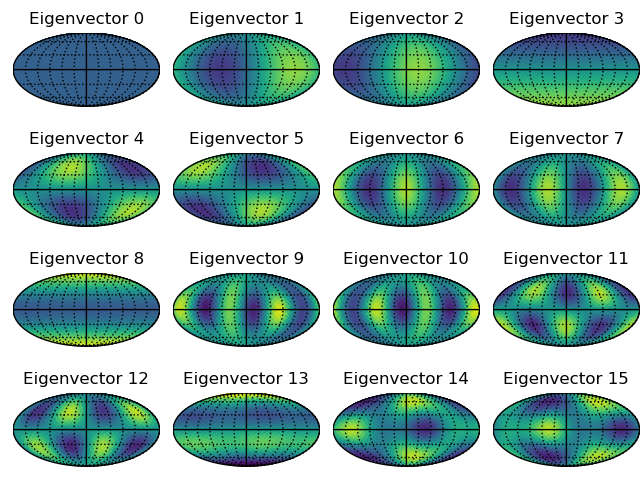
\includegraphics[width=0.6\textwidth]{../codes/03.FEM_laplacian/HEALPix/img/linear_FEM_8_eigenvectors.png}	
		\label{fig:spherical harmonics}
		\caption{The first 16 spherical harmonics}
	\end{figure}
	
	\item Of all the possible basis for $L^2(S^2)$ the spherical harmonics uniquely exploit the symmetries of the sphere. Under a rotation $g$, each spherical harmonic of degree $l$ is transformed into a linear combination of only those spherical harmonics of same degree $l$.
	Thus the effect of a rotation on a function expressed in the basis of the spherical harmonics is a multiplication by a semi-infinite block-diagonal matrix with the $(2l+1)\times(2l+1)$ blocks for each $l \geq 0$ given by $$D^{(l)}(g) = \left(D^{(l)}_{m,n}\right) (g) =  \left(D^{(l)}_{m,n}\right)(u(\phi)a(\theta)u(\psi)) = e^{-im\psi}d^{(l)}_{m,n}(\cos \theta) e^{-in\phi}$$
	The effect of all of this is to block-diagonalize rotationally invariant operators; namely, convolution operators obtained as weighted averages of the rotation operators by functions or kernels. For example the Laplace-Beltrami operator, that acts diagonally on the spherical harmonic basis.
	\item \begin{definition}{[\textit{Left Convolution}]}\\
		$k\star f(\omega) = \left(\int_{g\in SO(3)}dg\ k(g\eta)\Lambda(g)\right)f(\omega) = \int_{g\in SO(3)}k(g\eta)f(g^{-1}\omega)dg$
		where $\eta$ is the north pole. 
	\end{definition}
	Since the convolution is a linear combination of rotation operators $\Lambda(g)$, it follows that also the convolution must be block diagonalized. Indeed,
	$$\hat {(f \star h)}(l,m) = 2\pi \sqrt{\frac{4\pi}{2l+1}}\hat f(l,m) \hat h(l,0) $$

\end{enumerate}

\subsection{Spherical Convolutional Neural Networks}
[Review of \textit{Spherical CNNs}]
\subsection{Graph Spectral Theory} \label{sec:Chapter1: Spectral Graph Theory}
[Review of \textit{The emerging field of Graph Signal Processing}]
\subsection{Deep Sphere V1.0}
[Review of \textit{Deep Sphere}]
\subsection{Belkin's trinity}
[Review of \textit{the Belkin's trinity}]

\subsubsection{Towards a theoretical foundation of Laplacian-based manifold methods}
In this paper they present two results: a pointwise probabilistic convergence of \textbf{the extension of the graph Laplacian} 
\begin{definition}{Graph Laplacian}
	$$ \left(\mathbf L_n^t\right)_{ij}=\begin{cases}
	-w_{ij}, & i\neq j\\
	\sum_{k}w_{ik}, & i=j
	\end{cases}$$
\end{definition}
\begin{definition}{Point cloud Laplace operator}
	$$L_n^t:\quad(L_n^tf)(y) = \frac{1}{n}f(y)\sum_i e^{-\frac{||x_i-y||^2}{4t}}-\frac{1}{n}\sum_ie^{-\frac{||x_i-y||^2}{4t}}f(x_i)$$
\end{definition}
\begin{definition}{Functional approximation to the Laplace-Beltrami operator} \label{eq:L^t}
	$$L^tf(p) :=  \frac{1}{ (4\pi t)^{\frac{k+2}{2}}} \int_\mathcal Me^{-\frac{||p-x||^2}{4t}}\left(f(x)-f(p)\right)d\mu(x)$$
\end{definition}

\begin{theorem}{Pointwise convergence}
	$$\forall f \in C^\infty(\mathcal M)\quad  C\frac{(4\pi t_n)^{-\frac{k+2}{2}}}{n} L_n^t f(\bf x) \xrightarrow{n\to\infty}\triangle_\mathcal M f(\bf x)$$
\end{theorem}


and a uniform (pointwise convergence of the operator) one
\begin{theorem}{uniform convergence}
	$$\sup_{x\in\mathcal M, f\in \mathcal F_C}\left| C\frac{(4\pi t_n)^{-\frac{k+2}{2}}}{n} L_n^t f(\bf x) - \triangle_\mathcal M f(\bf x) \right|\xrightarrow{n\to\infty}0
	, \quad \mathcal F_C = \left\{f\in C^\infty(\mathcal M), f^{(i)}(x)\leq M, i=1,2,3\right\}$$
\end{theorem}


here nothing is said about convergence of the spectra, plus there's nothing written about the relationship between $\mathbf{Eig} L_n^t$ (the eigenfunctions and eigenvalues of the extension of the graph Laplacian) and $\mathbf {Eig} \mathbf {L}_n^t$ (the eigenvectors and eigenvalues of the matrix Laplacian).

Theorem 1 is proven by simple analysis arguments and by Hoeffding's formula (probability). 
First, by the simple law of large numbers, we have that for a fixed $t>0$, a fixed function $f$ and a fixed point $p\in\mathcal M$
\begin{equation}\label{eq:pointwise convergence of laplacian discrete approximation}
	\lim_{n\to\infty}\frac{1}{tn}\frac{1}{ (4\pi t)^{\frac{k}{2}}}L_n^tf(p)= L^tf(p)
\end{equation}




To prove the convergence of $L^t$ to $\triangle_\mathcal M$, then we need three steps, that we can recycle completely. They use the fact that thanks to the exponential map the heat kernel centered on $p$ on any manifold can be approximated by a Gaussian in the ambient Euclidean space in a small neighborhood of $p$, and the relationship between Euclidean distances and geodesic distances.

Theorem 2 is proven with arguments of Functional Analysis: Ascoli-Arzelà, compact convergence in Sobolev spaces, etc.etc...

\subsubsection{Consistency of Spectral Clustering}
$$ \mathbf{Eig} \mathbf{L}^t_n \xrightarrow[a.s.]{n\to\infty} \mathbf{Eig} L^t $$
It aims at proving the convergence of eigenvalues and eigenvectors of random graph Laplacian matrices for growing sample size. They present two results: one for the normalized Laplacian and one for the unnormalized Laplacian. Since the matrix eigenvectors grow in dimension as the sample size increases, standard convergence arguments can not be applied. However, they show that there exists a function $f\in C(\mathcal M)$ such that the difference between the eigenvector $v_n$ and the restriction of $f$ to the sample converges to $0$

$$||v_n-\rho_nf||\rightarrow 0$$

To do so they see the eigenvector $v_n$ as the restriction to the sample of a continuous eigenfunction $f_n$ of some continuous operator $U'_n$ that acts on the space $C(\mathcal M)$. Then they use the fact that 

$$||v_n-\rho_nf||_\infty = ||\rho_nf_n-\rho_nf||_\infty\leq ||f_n-f||_\infty$$


So, it will just be necessary to show that  $$||f_n-f||_\infty\rightarrow 0$$
\textbf{compact convergence} of both matrices towards $L^t$ (where $\mathcal M$ is a compact metric space) in the Banach space of the continuous functions $(C, ||\cdot||_\infty)$. 

Compact convergence ensures convergence of spectral properties in the following sense: for isolated eigenvalues of the limit operator $\triangle_\mathcal M$ with finite multiplicity we have convergence of eigenvalues and eigenspaces but not convergence of eigenfunctions. for isolated simple eigenvalues of the limit operator we have also convergence of the eigenfunctions!

The proof consists in three steps:
\paragraph{Step 1} Construct a bounded operator $U'_n$ on the Banach space $(C(\mathcal M), ||\cdot||_\infty)$ such that restricted on the sampled values behaves like $\mathbf{L}'_n$. Then, construct an operator $U'$ such that for the law of large numbers for a fixed $f$ and for a fixed $x$, $U'_nf(x) \xrightarrow U'f(x) $
\paragraph{Step 2} Here they establishes the connection between the spectra of $L'_n$ and $U'_n$. In particular, they prove a one-to-one correspondence between the eigenfunctions and eigenvalues of $U'_n$ and the eigenvectors and eigenvalues of $L'_n$, provided that satisfy $\lambda\notin \{1\}=\sigma_{ess}(U'_n)= \sigma_{ess}(U')$.
\paragraph{Step 3} Here we prove compact convergence:

$$U'_n \xrightarrow[n\to\infty]{c,\ a.s.}U'$$

At the light of compact convergence and on the analysis of the essential spectrum of $U'_n, U'$ and the one-to-one correspondence of the spectra done in step 2, given Proposition 6 \textit{Perturbation results for compact convergence} we get to the following result

\begin{theorem}
	Let $\lambda\neq 1 $ be an eigenvalue of $U'$ and $M\subset \mathbb C$ an open neighborhood of $\lambda$ such that $\sigma(U')\cap M=\{\lambda\}$. Then:
	\begin{enumerate}
		\item Convergence of eigenvalues: The eigenvalues in$\sigma(L'_n)\cap M$ converge to $\lambda$ in the sense that every sequence $(\lambda_n)_{n\in\mathbb N}$ with $\lambda_n\in\sigma(L'_n)\cap M$ satisfies $\lambda_n\rightarrow \lambda$ almost surely.
		\item Convergence of spectral projections: There exists some $N\in\mathbb N$ such that for $n>N$, the sets $\sigma(U'_n)\cap M$ are isolated in $\sigma(U'_n)$. For $n>N$, let $Pr'_n$ be the spectral projection of $U'_n$ corresponding to $\sigma(U'_n)\cap M$, and $Pr$ the spectral projection of $U$ for $\lambda$. Then $Pr'_n\xrightarrow p Pr a.s.$
		\item Convergence of eigenvectors: if $\lambda$ is a single eigenvalue, then the eigenvectors of $L'_n$ converge a.s. up to a change of sign: if $v_n$ is the eigenvector
		of $L'_n$ with eigenvalue $\lambda_n$, $v_{n,i}$ its i-th coordinate, and $f$ the eigenfunction of eigenvalue $\lambda$, then there exists a sequence $(a_n)_{n\in\mathbb N}$ with $a_i \in \{+1,-1\}$ such that $\sup_{i=1,...,n} |a_nv_{n,i} - f(X_i)| \rightarrow 0$ a.s. In particular, for all $b \in\mathbb R$, the sets $\{a_nf_n > b\}$ and $\{f > b\}$ converge, that is, their symmetric difference satisfies $P(\{f > b\}\triangle\{a_nf_n > b\}) \rightarrow 0$.
	\end{enumerate}
\end{theorem}

A similar theorem is stated also for non-normalized Laplacian matrix, although the arguments stay the same.
\subsubsection{Convergence of Laplacian Eigenmaps}
Here all the pieces are put together. 

$$ \mathbf{Eig} \mathbf{ L}^t_n \xrightarrow[a.s.]{n\to\infty} \mathbf{Eig} L^t \xrightarrow{t\to0} \mathbf{Eig} \triangle_\mathcal M $$

\begin{theorem}
	Let $\lambda_{n,i}^t$ be the ith eigenvalue of $\hat L_n^t$ and $e^t_{n,i}$ be the corresponding eigenfunction (which for each fixed i will be shown to exist for t sufficiently small). Let $\lambda_{i}$ be the ith eigenvalue of $\triangle_\mathcal M$ and $e_{i}$ be the corresponding eigenfunction. Then there exists a sequence $t_n\rightarrow 0$ such that
	
	$$\lim_{n\rightarrow\infty} \lambda_{n,i}^{t_n}=\lambda_i$$
	$$\lim_{n\rightarrow\infty}||e_{n,i}^{t_n}(x) - e_i(x)||_2 = 0$$
	
	where the limits are in probability.
	
\end{theorem}

\paragraph{Step 1: Spectral convergence of the empirical approximation $\mathbf{ L}_n^t$ to $L^t$}
Recycle the work of \textbf{Consistency of Spectral Clustering} with the analysis of the essential spectrum of the limit operator $\sigma_{ess}(L^t)$.
\paragraph{Step 2: Spectral convergence of the functional approximation $L^t$ to $\triangle$}
Really hard. Uniform operator convergence does not hold, however spectral convergence is still assured in theorem 4.1 of the paper. This part, although really hard, will stay the same!
sub